\section{Dérivée $k^{ième}$}
Soit \il{x} une liste d'abscisses de $a$ à $b$ inclus avec un \il{pas} constant.
On pose $y = f(x)$.\\
\q{Par récursivité, construire un fonction }\il{deriveekieme(y, x, k)}\q{ qui
  calcule la dérivée $k^{ième}$ de }\il{y}\q{ par rapport à }\il{x}\q{.
  Elle retournera une liste de longueur }\il{len(x)-k}\q{.}

\codeFromFileT{main.py}{section-02/q1-1.py}

\begin{enumerate}[(a)]
  \item On pose $f(x) = sin(x)$, $a = 0$, $b=6$ et $n = 1000\times$\il{pas}.\\
        \q{Tracer les graphes en valeur absolue des dérivées $k^{ième}$ de $f$
        pour $k \in [\![1, 6]\!]$.}\\

        \codeFromFileT{main.py}{section-02/q1-2.py}

        \il{TraceDeriv(f, 0, 6, 1000)} donne :

        \begin{center}
          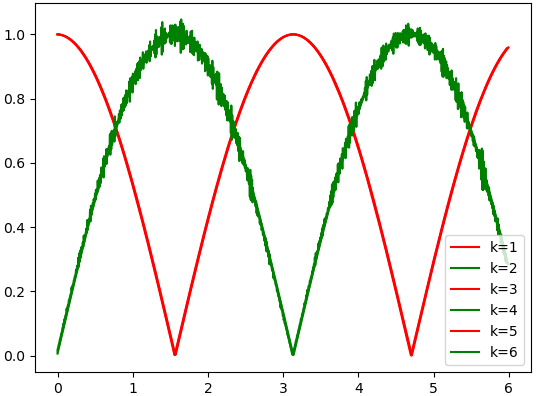
\includegraphics[scale=0.5]{section-02/q1-3.png}
        \end{center}

        \q{Peut-on le faire pour $k=7$ ?}
        \begin{center}
          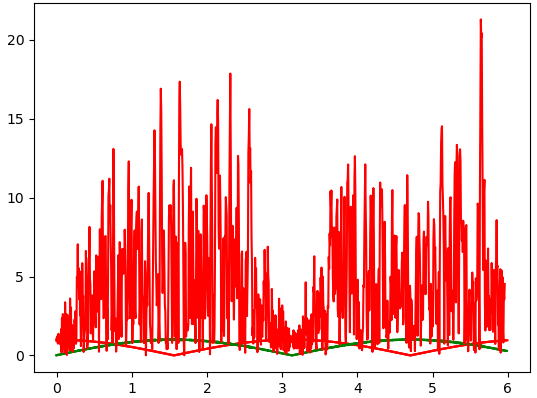
\includegraphics[scale=0.5]{section-02/q1-4.png}
        \end{center}
        Oui, mais ça ne donne pas la dérivée $7^{i\grave{e}me}$ !
  \item\q{Que faut-il contrôler pour que la fonction }\il{deriveekieme}\q{ donne
          un résultat correct ?}\\
        Il faut que l'odre de la dérivée ne soit pas trop grand...
\end{enumerate}
